\begin{frame}
	\frametitle{O sistema 10-20 de posicionamento de eletrodos}
	\begin{columns}
		\begin{column}{0.3\textwidth}
			\par De acordo com \cite{ScienceOpenVid:5960cfa8-7fde-441c-8592-35fdb9841499} os eletrodos responsáveis pela captação do sinal devem ser dispostos segundo um espaçamento de 20\% do tamanho da cabeça do paciente respeitando-se uma 'margem' de 10\% em relação ao \textit{nasion}, \textit{inion} e ao ponto pré-auricular.
		\end{column}
		\begin{column}{0.7\textwidth}
			\begin{figure}
				\centering
				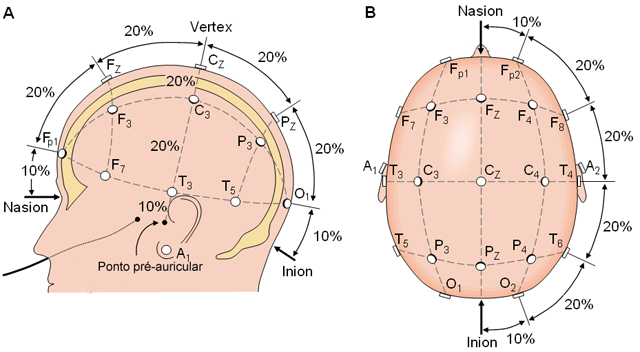
\includegraphics[width=\linewidth]{images/sistema10-20}
				\caption{Ilustração do sistema 10-20 fonte: \cite{sistema10-20}}
				\label{fig:sistema10-20}
			\end{figure}
		\end{column}
	\end{columns}
\end{frame}